\subsection{Results and discussion}


%%%%%%%%%%%%%%%%%%%%%%%%%%%%%%%%%%%%%%%%%%%%%%%%%%%%%%%%%%%%%%%%
%%  Systematic quant. of the relationship between stereo. and small molecule bioactivity
%%%%%%%%%%%%%%%%%%%%%%%%%%%%%%%%%%%%%%%%%%%%%%%%%%%%%%%%%%%%%%%%

\phantomsection
\subsubsection{Systematic quantification of the relationship between stereochemistry and small molecule bioactivity}
\label{Stereoisomers_Rel_Stereo_Bioactivity}


% The first steps in the development of Signaturizers3D were (i) to select a comprehensive database containing detailed bioactivity data for a wide range of chemical compounds, and (ii) within this database, systematically identify groups of stereoisomers to compare their bioactivity profiles and evaluate the ability of Signaturizers3D to distinguish them.
% To gather bioactivity data, we used the Chemical Checker (CC), which represents the largest collection of small molecule bioactivity signatures available to date, with experimental information for over 1M compounds [6]. The CC divides data into five levels of increasing complexity, ranging from the chemical properties of compounds to their clinical outcomes. Compound bioactivities are expressed in a vector-like format (i.e. signatures), and the data processing pipeline also includes several steps of increasing level of integration and abstraction: from raw experimental data representing explicit knowledge (type 0 signatures) to inferred representations that leverage all the experimentally determined bioactivities available for each molecule (type III signatures). Thus, we processed the whole CC (i.e. 25 different bioactivity types for about 1M molecules) to systematically identify groups of stereoisomers that might exhibit distinct bioactivities. In brief, we first identified stereoisomers using their InChIKey strings and we then applied several filters to ensure that the actual differences between compounds were exclusively due to stereochemical variations (see Supplementary Information for further details). Then, we selectively removed molecules that were not exhaustively characterized, in order to work with enantiomerically pure compounds and prevent the analysis of results derived from racemic mixtures (Fig 1a). We eventually identified 23,830 groups of stereoisomers, involving 57,989 compounds, across the different CC bioactivity spaces. We found most stereoisomeric groups with experimental information in the target binding space (B4) and in the network spaces derived from B4 (i.e. C3-5, Fig S1). We thus focused our study on the B4 space, which contains over 600,000 molecules, and we identified 15,370 groups of stereoisomers, involving 32,705 compounds (Fig 1b). We then analyzed the binding profiles for all these compounds, and found 6,022 groups that had at least 2 stereoisomers with non-identical binding profiles. We also observed that the majority of the groups (14,181, ~92%) contained only 2 stereoisomers (Fig 1c, top), in 38% of which both compounds showed distinct binding profiles (Fig 1c, bottom). Analogously, we identified 562 groups containing 3 stereoisomers: 230 (41%), 195 (35%) and 137 (24%) of them showing 1, 2 and 3 distinct binding profiles, respectively. Finally, we observed that the distribution of Jaccard distances between binding profiles within stereoisomeric groups was skewed towards low values (i.e. more similar profiles) compared with random pairs, while pairs of compounds sharing at least one target were somewhere in the middle (Fig 1d). Fig 1e shows, as an illustrative example, a group of 3 stereoisomers with non-identical binding profiles, where compounds A and C weakly and strongly bind with the Beta-1 adrenergic receptor (ADRB1; 2nd position in the profile), respectively, whilst compound B does not bind it. Note that inactive compound-target interactions might be false negatives due to, for instance, a limited sensitivity of the detection methods or non-tested enantiomers.


\begin{Figure_modified}
  \centering
  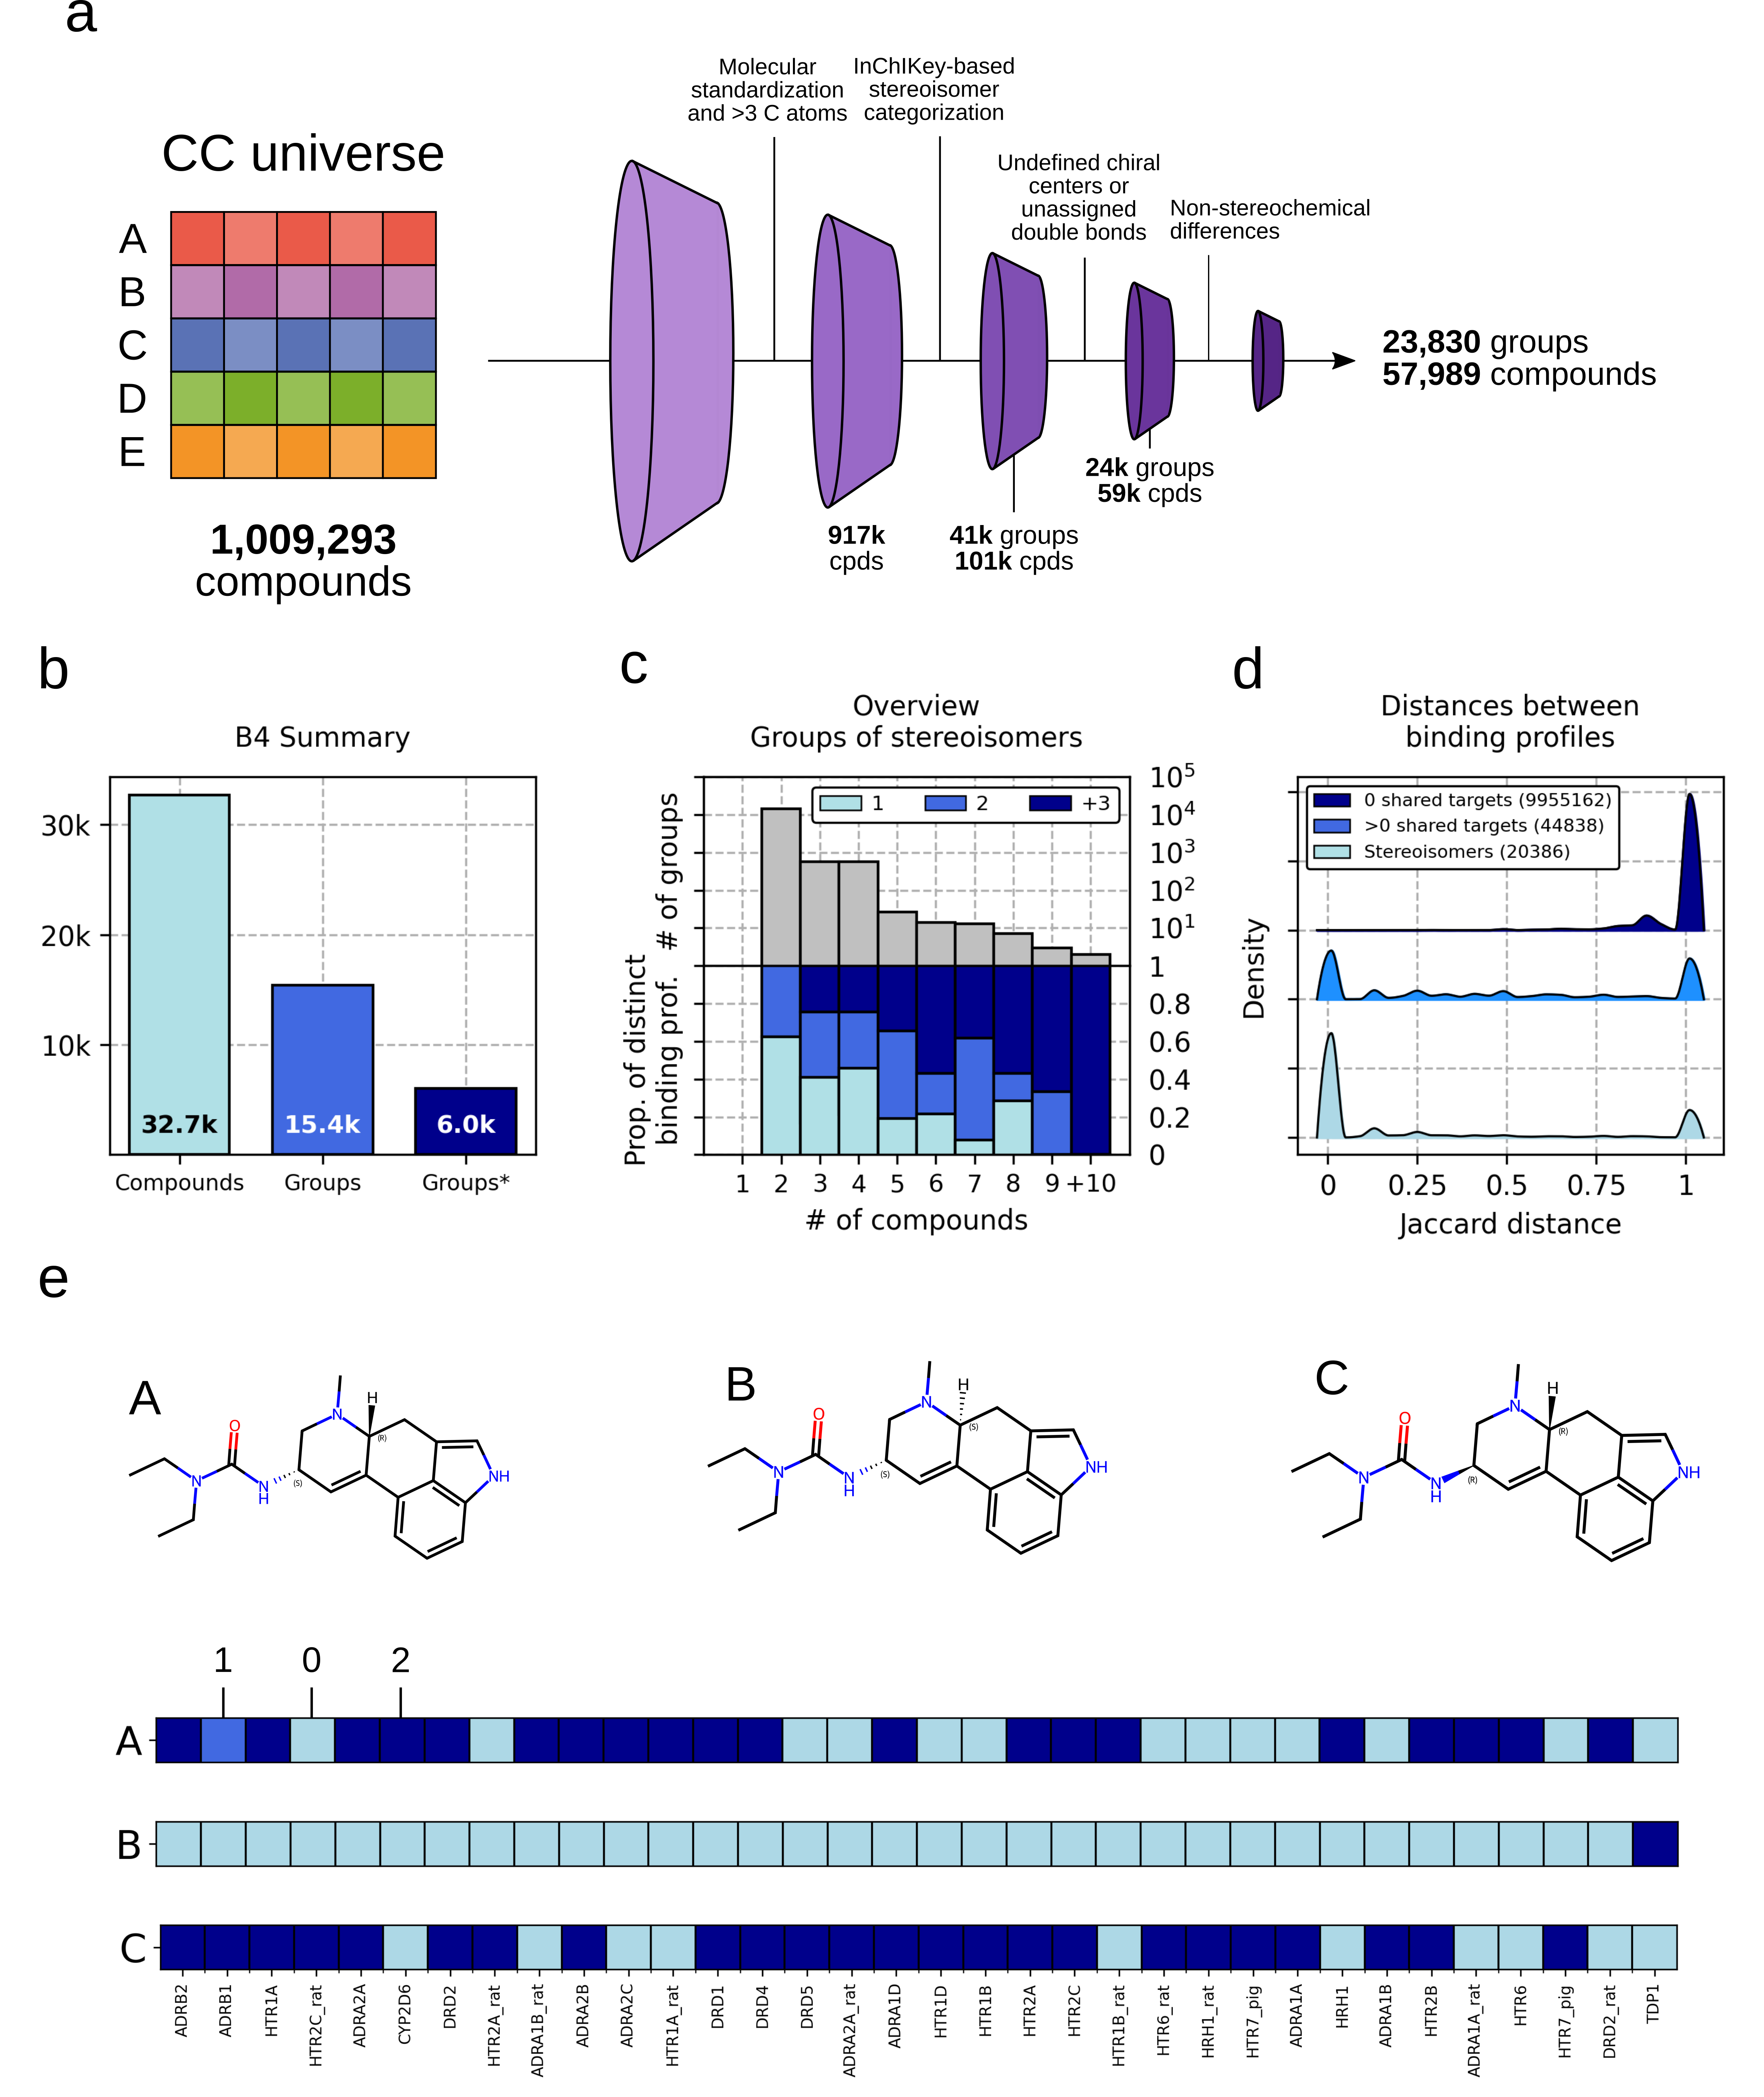
\includegraphics[width=1\linewidth]{figures/Stereoisomers/Main/Fig1_v2.png}
  \caption{
    \textbf{Stereoisomerism and bioactivity.}
    \textbf{a)} Computational pipeline to identify groups of stereoisomers in the CC chemical universe.
    \textbf{b)} Number of unique stereoisomeric compounds with experimentally identified protein targets in the CC B4 space, number of stereoisomer groups, and number of groups with at least 2 compounds with non-identical binding profiles.
    \textbf{c)} Number of groups (y-axis, top) having the specified number of stereoisomers (x-axis). Proportion of these groups (y-axis, bottom) having the specified number of distinct binding profiles (i.e. \textasciitilde60\% of the groups of 2 isomers have a unique binding profile).
    \textbf{d)} Distributions of Jaccard distances (binding profiles) between pairs of compounds sharing 0, ≥1 targets and stereoisomer pairs. All distributions are significantly different from each other (Mann-Whitney p-value\textasciitilde0).
    \textbf{e)} Illustrative example of a stereoisomer group including 3 small molecules with their corresponding target binding profiles, using the annotation of type 0 signatures (i.e. 0: no binding; 1: weak binding and 2: strong binding).
    \rule[0ex]{\textwidth}{0.5pt}
  }
  \label{Stereoisomers_Fig1}
\end{Figure_modified}